\documentclass[11pt]{article}
\usepackage[utf8]{inputenc}	% Para caracteres en español
\usepackage[hidelinks]{hyperref}
\usepackage{amsmath,amsthm,amsfonts,amssymb,amscd}
\usepackage{multirow,booktabs}
\usepackage[table]{xcolor}
\usepackage{fullpage}
\usepackage{lastpage}
\usepackage{enumitem}
\usepackage{fancyhdr}
\usepackage{mathrsfs}
\usepackage{wrapfig}
\usepackage{setspace}
\usepackage{calc}
\usepackage{multicol}
\usepackage{cancel}
\usepackage[10pt]{extsizes}
\usepackage{amsfonts}
\usepackage{amsthm}
\usepackage{amssymb}
\usepackage[margin=3cm]{geometry}
\usepackage{amsmath}
\newlength{\tabcont}
\usepackage{empheq}
\usepackage{framed}
\usepackage[most]{tcolorbox}
\usepackage{xcolor}
\colorlet{shadecolor}{orange!15}
\parindent 0in
\parskip 12pt
\theoremstyle{definition}
\newtheorem{defn}{Definition}
\newtheorem{reg}{Rule}
\newtheorem{exer}{Exercise}
\newtheorem{note}{Note}
\allowdisplaybreaks[4]

\newcommand{\Z}{\mathbb{Z}}
\newcommand{\R}{\mathbb{R}}
\newcommand{\C}{\mathbb{C}}
\newcommand{\F}{\mathbb{F}}
\newcommand{\E}{\mathbb{E}}
\newcommand{\bigO}{\mathcal{O}}
\newcommand{\Real}{\mathcal{Re}}
\newcommand{\poly}{\mathcal{P}}
\newcommand{\mat}{\mathcal{M}}
\DeclareMathOperator{\Span}{span}
\newcommand{\Hom}{\mathcal{L}}
\DeclareMathOperator{\Null}{null}
\DeclareMathOperator{\Range}{range}
\newcommand{\defeq}{\vcentcolon=}
\newcommand{\restr}[1]{|_{#1}}

\begin{document}
\setcounter{section}{0}
\title{Chapter 1 Review Notes}

\thispagestyle{empty}

% Problem environment

\newtcbtheorem{prob}% environment name
              {Problem}% Title text
  {enhanced, % tcolorbox styles
  attach boxed title to top left={xshift = 4mm, yshift=-2mm},
  colback=blue!5, colframe=black, colbacktitle=blue!3, coltitle=black,
  boxed title style={size=small,colframe=gray},
  fonttitle=\bfseries,
  separator sign none
  }%
  {} 
\newenvironment{problem}[1]{\begin{prob*}{#1}{}}{\end{prob*}}

\begin{center}
{\LARGE \bf Chapter 1: Introduction}\\
{\large Notes for Pattern Recognition and Machine Learning by Christopher Bishop}\\
\end{center}

\setcounter{tocdepth}{2}
\tableofcontents
% \newpage
% \section{Note}
% \subsection{fitting}
% \newpage

\setcounter{secnumdepth}{1}
\section{Exercises}

\subsection{Exercise 1.1}
\begin{proof}
According to Eq. (1.2), we can get the error function:
\begin{equation*}
E(\bold{w}) = \frac{1}{2}\sum^{N}_{n=1} \{ y\left(x_n,\bold{w}\right) - t_n \}.
\end{equation*}
Calculating the derivative of this function with respect to $w_i$ we can get:
\begin{equation}
 \frac{\partial E(\bold{w})}{\partial w_i} = \sum^{N}_{n=1}x_n\{y\left(x_n,\bold{w}\right) - t_n\}.  \label{eq:eq1} 
\end{equation}
Let Eq. (\ref{eq:eq1}) equals to 0, then
\begin{equation*}
\begin{aligned}
\sum^{N}_{n=1}x_n\{y\left(x_n,\bold{w}\right) - t_n\} &= 0 \\
\Rightarrow\sum^N_{n=1}y(x_n,\bold{w})x_n^i &= \sum^N_{n=1}t_nx_n^i \\
\Rightarrow\sum^N_{n=1}\{x_n^i(\sum^M_{j=0}w_jx_n^j)\} &= \sum^N_{n=1}t_nx_n^i \\
\Rightarrow\sum^N_{n=1}\sum^M_{j=0}w_j(x_n)^{i+j} &= \sum^N_{n=1}t_nx_n^i \\
\Rightarrow\sum^M_{j=0}\sum^N_{n=1}w_j(x_n)^{i+j} &= \sum^N_{n=1}t_nx_n^i.
\end{aligned}
\end{equation*}
According to Eq. (1.122) and (1.123), we can get
\begin{equation*}
\begin{aligned}
\sum^M_{j=0}\sum^N_{n=1}w_j(x_n)^{i+j} &= \sum^N_{n=1}t_nx_n^i \\
\Rightarrow\sum^M_{j=0}\{\sum^N_{n=1}(x_n)^{i+j}\}w_j &= \sum^N_{n=1}t_nx_n^i \\
\Rightarrow\sum^M_{j=0}A_{ij}w_j &= T_i,
\end{aligned}
\end{equation*}
as desired.
\end{proof}

\subsection{Exercise 1.2}
\begin{proof}
According to Eq. (1.4), we can get the error function:
\begin{align*}
\widetilde{E}(\bold{w}) = \frac{1}{2}\sum^{N}_{n=1} \{ y\left(x_n,\bold{w}\right) - t_n \} + \frac{\lambda}{2}\lVert\bold{w}\rVert^2_2.
\end{align*}
Calculating the derivative of this function with respect to $w_i$ we can get:
\begin{align}
\frac{\partial \widetilde{E}(\bold{w})}{\partial w_i} = \sum^{N}_{n=1}x_n\{y\left(x_n,\bold{w}\right) - t_n\} + \lambda w_i.  \label{eq:eq2}   
\end{align}
Let Eq. (\ref{eq:eq2}) equals to 0, then
\begin{align}
\lambda w_i + \sum^{N}_{n=1}x_n\{y\left(x_n,\bold{w}\right) - t_n\} &= 0 \nonumber\\
\Rightarrow\lambda w_i +  \sum^N_{n=1}y(x_n,\bold{w})x_n^i &= \sum^N_{n=1}t_nx_n^i \nonumber\\
\Rightarrow\lambda w_i +   \sum^M_{j=0}\{\sum^N_{n=1}(x_n)^{i+j}\}w_j &= \sum^N_{n=1}t_nx_n^i \nonumber\\
\Rightarrow\sum^M_{j=0}\{\sum^N_{n=1}(x_n)^{i+j}+\lambda\mathbb{I}_{(i=j)}\}w_j &= \sum^N_{n=1}t_nx_n^i, \label{eq:eq3}
\end{align}
where $\mathbb{I}_{(i=j)} = 1$ if and only if $i=j$, otherwise 0.
According to Eq. (\ref{eq:eq3}), (1.122) and (1.123), we can rewrite similar set of equations
\begin{equation*}
\begin{aligned}
\sum^{M}_{j=0}A_{ij}w_j = T_i,
\end{aligned}
\end{equation*}
where
\begin{equation*}
\begin{aligned}
A_{ij} = \sum^N_{n=1}\{(x_n)^{i+j}+\lambda\mathbb{I}_{(i=j)}\},\  T_i = \sum^N_{n=1}(x_n)^it_n.
\end{aligned}
\end{equation*}
\end{proof}

\subsection{Exercise 1.3}
\begin{proof}
We suppose that the probability of selecting an apple from boxes is $p(a)$, then
\begin{align*}
p(a) = p(a|r)p(r) + p(a|b)p(b) + p(a|g)p(g) = 0.34.
\end{align*}
Suppose that the probability of selecting an orange from boxes is $p(o)$. There is an equation
\begin{align*}
p(og) = p(o|g)p(g) = p(g|o)p(o).
\end{align*}
Hence we can get
\begin{align*}
p(g|o) = \frac{p(o|g)p(g)}{p(o)} = \frac{p(o|g)p(g)}{p(o|r)p(r) + p(o|b)p(b) + p(o|g)p(g)} = 0.5.
\end{align*}
\end{proof}

\subsection{Exercise 1.4}
\begin{proof}
According to Eq. (1.27), we can get
\begin{align*}
p_y(y) = p_x(g(y))|g'(y)|.
\end{align*}
By differentiating Eq. (1.27), we can get
\begin{align}
\frac{dp_y(y)}{dy} &= \frac{dp_x(g(y))|g'(y)|}{dy} \nonumber\\
&= |g'(y)|\frac{dp_x(g(y))}{dy} + 
 p_x(g(y))\frac{d|g'(y)|}{dy}. \label{eq:eq4}
\end{align}
Calculating the derivative of $p_x(x)$, it is obvious that it equals to 0 when $x=\hat{x}$, so
\begin{align*}
{\left.{\frac{dp_x(x)}{dx}}\right|}_{\hat{x}} = 0.
\end{align*}
When $g(y) = \hat{x}$, Eq. (\ref{eq:eq4}) is equivalent to
\begin{align}
\frac{dp_y(y)}{dy}  &= |g'(y)|\frac{dp_x(g(y))}{dy} + 
 p_x(g(y))\frac{d|g'(y)|}{dy} \nonumber\\
 &= |g'(y)|\frac{dp_x(g(y))}{dg(y)}\frac{dg(y)}{dy} + 
 p_x(g(y))\frac{d|g'(y)|}{dy}\nonumber\\
 &= |g'(y)|\cdot 0 \cdot\frac{dg(y)}{dy} + 
 p_x(g(y))\frac{d|g'(y)|}{dy}\nonumber\\
 &= p_x(g(y))\frac{d|g'(y)|}{dy},\nonumber
\end{align}
 Equation $p_x(g(y))\frac{d|g'(y)|}{dy}$ is always 0 means that if $\hat{x}$ is the location of the maximum of $p_x(x)$, $\hat{y}$, where $g(\hat{y}) = \hat{x}$, is also the location of the maximum of $p_y(y)$. By observing the last term $p_x(g(y))\frac{d|g'(y)|}{dy}$, $p_x(g(y))$ is a density probability hence it is not always 0. $\frac{d|g'(y)|}{dy} = 0$, if and only if $g(y)$ is a linear function, which means in the case of a linear transformation, the location of the maximum transforms in the same way as the variable itself, as desired.
\end{proof}

\subsection{Exercise 1.5}
\begin{proof}
\begin{align*}
var[f] &= \mathbb{E}\left[(f(x)-\mathbb{E}[f(x)])^2\right] \\
&= \mathbb{E}\left[f(x)^2 - 2f(x)\mathbb{E}[f(x)] + \mathbb{E}[f(x)]^2\right] \\
&= \mathbb{E}[f(x)^2] - 2\mathbb{E}[f(x)]\E[f(x)] + \mathbb{E}[f(x)]^2 \\
&= \mathbb{E}[f(x)^2] - 2\mathbb{E}[f(x)]^2 + \mathbb{E}[f(x)]^2\\
&= \mathbb{E}[f(x)^2] - \mathbb{E}[f(x)]^2,
\end{align*} 
as desired.
\end{proof}

\subsection{Exercise 1.6}
\begin{proof}
If $x, y$ are discrete independent variables, they follow
\begin{align}
\mathbb{E}_{x,y}[xy] &= \sum_{x}\sum_{y}p(xy)xy \nonumber\\
&= \sum_{x}\sum_{y}xyp_x(x)p_y(y) \nonumber\\
&= \sum_{x}xp_x(x)\sum_{y}yp_y(y) \nonumber\\
&= \mathbb{E}[x]\mathbb{E}[y]. \label{eq:eq5}
\end{align}
If $x, y$ are continuous independent variables, they follow
\begin{align}
\mathbb{E}_{x,y}[xy] &= \int_{x}\int_{y}p(xy)xydxdy \nonumber\\
&= \int_{x}\int_{y}xyp_x(x)p_y(y)dxdy \nonumber\\
&= \int_{x}xp_x(x)dx\int_{y}yp_y(y)dy \nonumber\\
&= \mathbb{E}[x]\mathbb{E}[y]. \label{eq:eq6}
\end{align}
With the combination of Eq. (\ref{eq:eq5}) and (\ref{eq:eq6}), we can get that if $x, y$ are independent variables, they satisfy
\begin{align}
\mathbb{E}_{x,y}[xy] = \mathbb{E}[x]\mathbb{E}[y]. \nonumber
\end{align}
Hence $cov[x, y]$ follows
\begin{equation*}
\begin{aligned}
cov[x, y] &= \mathbb{E}_{x,y}\left[\{x-\mathbb{E}[x]\}\{y-\mathbb{E}[y]\}\right] \\
&= \mathbb{E}_{x,y}[xy] - \mathbb{E}[x]\mathbb{E}[y] \\
&= \mathbb{E}[x]\mathbb{E}[y] - \mathbb{E}[x]\mathbb{E}[y] \\
&= 0,
\end{aligned}
\end{equation*}
as desired.
\end{proof}

\subsection{Exercise 1.7}
\begin{proof}
According to Eq. (1.125), we have
\begin{align*}
I^2 =& \int^{+\infty}_{-\infty}\int^{+\infty}_{-\infty}\exp\left(-\frac{1}{2\sigma^2}(x^2+y^2)\right)dxdy\\
&= \int^{2\pi}_{0}\int^{\infty}_{0}\exp\left(-\frac{1}{2\sigma^2}r^2\right)rdrd\theta\\
&= \frac{1}{2}\int^{2\pi}_{0}\int^{\infty}_{0}\exp\left(-\frac{1}{2\sigma^2}r^2\right)dr^2d\theta\\
&= -\sigma^2\int^{2\pi}_{0}\int^{\infty}_{0}\exp\left(-\frac{1}{2\sigma^2}r^2\right)d\left(-\frac{1}{2\sigma^2}\right)r^2d\theta\\
&=\sigma^2\int^{2\pi}_{0}d\theta\\
&= 2\pi\sigma^2,
\end{align*}
where we apply $x = rcos\theta, y = rsin\theta$. Thus $I = (2\pi\sigma^2)^{\frac{1}{2}}$. Then
\begin{align*}
\int^{+\infty}_{-\infty}\mathcal{N}\left(x|\mu,\sigma^2\right)dx &= \int^{+\infty}_{-\infty}\frac{1}{(2\pi\sigma^2)^{\frac{1}{2}}}\exp\left\{-\frac{1}{2\sigma^2}\left(x-\mu\right)^2\right\}dx\\
&= \frac{1}{(2\pi\sigma^2)^{\frac{1}{2}}}\int^{+\infty}_{-\infty}\exp\left\{-\frac{1}{2\sigma^2}\left(x-\mu\right)^2\right\}d(x-\mu)\\
& = \frac{1}{(2\pi\sigma^2)^{\frac{1}{2}}}(2\pi\sigma^2)^{\frac{1}{2}} = 1,
\end{align*}
as desired.
\end{proof}

\subsection{Exercise 1.8}
\begin{proof}
\begin{align*}
\E[x] &= \int^{+\infty}_{-\infty}\mathcal{N}\left(x|\mu,\sigma^2\right)xdx = \int^{+\infty}_{-\infty}\frac{x}{(2\pi\sigma^2)^{\frac{1}{2}}}\exp\left\{-\frac{1}{2\sigma^2}\left(x-\mu\right)^2\right\}dx\\
&= \int^{+\infty}_{-\infty}\frac{(x-\mu+\mu)}{(2\pi\sigma^2)^{\frac{1}{2}}}\exp\left\{-\frac{1}{2\sigma^2}\left(x-\mu\right)^2\right\}dx\\
&= \int^{+\infty}_{-\infty}\frac{(x-\mu)}{(2\pi\sigma^2)^{\frac{1}{2}}}\exp\left\{-\frac{1}{2\sigma^2}\left(x-\mu\right)^2\right\}d(x-\mu) +  \int^{+\infty}_{-\infty}\frac{\mu}{(2\pi\sigma^2)^{\frac{1}{2}}}\exp\left\{-\frac{1}{2\sigma^2}\left(x-\mu\right)^2\right\}d(x-\mu)\\
&= 0 + \frac{\mu}{(2\pi\sigma^2)^{\frac{1}{2}}}(2\pi\sigma^2)^{\frac{1}{2}}\\
&= \mu,
\end{align*}
as desired.
\begin{equation*}
\begin{aligned}
\E[x^2] &= \int^{+\infty}_{-\infty}\mathcal{N}\left(x|\mu,\sigma^2\right)x^2dx = \int^{+\infty}_{-\infty}\frac{x^2}{(2\pi\sigma^2)^{\frac{1}{2}}}\exp\left\{-\frac{1}{2\sigma^2}\left(x-\mu\right)^2\right\}dx\\
&= \int^{+\infty}_{-\infty}\frac{(x-\mu)^2+2\mu x - \mu^2}{(2\pi\sigma^2)^{\frac{1}{2}}}\exp\left\{-\frac{1}{2\sigma^2}\left(x-\mu\right)^2\right\}dx\\
&= \int^{+\infty}_{-\infty}\frac{(x-\mu)^2}{(2\pi\sigma^2)^{\frac{1}{2}}}\exp\left\{-\frac{1}{2\sigma^2}\left(x-\mu\right)^2\right\}dx\\ &+ 2\mu \int^{+\infty}_{-\infty}\frac{x}{(2\pi\sigma^2)^{\frac{1}{2}}}\exp\left\{-\frac{1}{2\sigma^2}\left(x-\mu\right)^2\right\}dx\\ & - \int^{+\infty}_{-\infty}\frac{\mu^2}{(2\pi\sigma^2)^{\frac{1}{2}}}\exp\left\{-\frac{1}{2\sigma^2}\left(x-\mu\right)^2\right\}dx\\
&= \int^{+\infty}_{-\infty}\frac{(x-\mu)^2}{(2\pi\sigma^2)^{\frac{1}{2}}}\exp\left\{-\frac{1}{2\sigma^2}\left(x-\mu\right)^2\right\}dx\\ &+ 2\mu \int^{+\infty}_{-\infty}\frac{x}{(2\pi\sigma^2)^{\frac{1}{2}}}\exp\left\{-\frac{1}{2\sigma^2}\left(x-\mu\right)^2\right\}dx -\mu^2\\
&= \int^{+\infty}_{-\infty}\frac{(x-\mu)^2}{(2\pi\sigma^2)^{\frac{1}{2}}}\exp\left\{-\frac{1}{2\sigma^2}\left(x-\mu\right)^2\right\}dx + 2\mu \int^{+\infty}_{-\infty}\frac{x}{(2\pi\sigma^2)^{\frac{1}{2}}}\exp\left\{-\frac{1}{2\sigma^2}\left(x-\mu\right)^2\right\}dx-\mu^2\\
&=\int^{+\infty}_{-\infty}\frac{(x-\mu)^2}{(2\pi\sigma^2)^{\frac{1}{2}}}\exp\left\{-\frac{1}{2\sigma^2}\left(x-\mu\right)^2\right\}d(x-\mu) + \mu^2\\
&= \frac{1}{(2\pi\sigma^2)^{\frac{1}{2}}}\int^{+\infty}_{-\infty}(x-\mu)^2\exp\left\{-\frac{1}{2\sigma^2}\left(x-\mu\right)^2\right\}d(x-\mu) + \mu^2\\
&= \frac{\sqrt{2}\sigma \cdot 2\sigma^2}{\sqrt{2\pi}\sigma}\int^{+\infty}_{-\infty}\left(\frac{x-\mu}{\sqrt{2}\sigma}\right)^2\exp\left\{-\left(\frac{x-\mu}{\sqrt{2}\sigma}\right)^2\right\}d\left(\frac{x-\mu}{\sqrt{2}\sigma}\right) + \mu^2\\
&= \frac{\sqrt{2}\sigma \cdot 2\sigma^2}{\sqrt{2\pi}\sigma} \cdot \frac{\sqrt{\pi}}{2} + \mu^2\\
&= \mu^2 + \sigma^2,
\end{aligned}
\end{equation*}
where we utilize $\int^{+\infty}_{-\infty}x^2\exp(-x^2)dx = \frac{\sqrt{\pi}}{2}$ [\href{https://math.stackexchange.com/questions/66084/integral-int-infty-infty-x2-e-x2-mathrm-dx}{Proof}]. Hence we have $var[x] = \E[x^2] - \E[x]^2 = \sigma^2$.
\end{proof}

\subsection{Exercise 1.9}
\begin{proof}
Let us get the derivative of $\mathcal{N}(x|\mu, \sigma^2)$
\begin{equation*}
\frac{\partial\mathcal{N}(x|\mu, \sigma^2)}{\partial x} =  -\frac{2(x-\mu)}{\sqrt{2\pi}\sigma}\exp\left\{-\frac{1}{2\sigma^2}\left(x-\mu\right)^2\right\}.
\end{equation*}
Obviously, $\mathcal{N}(x|\mu, \sigma^2)$ is monotonically increasing on the interval $(-\infty, \mu)$ and decreasing on the interval $(\mu, +\infty)$. Hence mode (i.e. the maximum) of the univariate Gaussian distribution is given by $\mu$.\\
For multivariate Gaussian distribution, we can get its derivative [\href{https://www.matrixcalculus.org/}{Matrix Calculus}]
\begin{equation*}
\frac{\partial\mathcal{N}(\bf x|\boldsymbol{\mu}, \bf\Sigma)}{\partial \bf x} = -\frac{1}{2}\mathcal{N}(\bf x|\boldsymbol{\mu})(\bf \Sigma^{-1} + (\bf {\Sigma^{-1}})^{T})(\bf x - \boldsymbol{\mu}).
\end{equation*}
Hence we have $\frac{\partial\mathcal{N}(\bf x|\boldsymbol{\mu}, \bf\Sigma)}{\partial \bf x} = 0$ when $\bf x = \boldsymbol{\mu}$. Thus the mode of the multivariate Gaussian is given by $\boldsymbol{\mu}$.
\end{proof}

\subsection{Exercise 1.10}
\begin{proof}
If $x, z$ are continuous independent variables, we have
\begin{align*}
\E[x+z] &= \int_z\int_x (x+z)p(x,z)dxdz\\
&= \int_z\int_x (x+z)p(x)p(z)dxdz\\
&= \int_z\int_x xp(x)p(z) + zp(x)p(z)dxdz\\
&= \int_z\int_x xp(x)p(z)dxdz + \int_z\int_x zp(x)p(z)dxdz\\
&= \int_z p(z)dz\int_x xp(x)dx + \int_x p(x)dx\int_z zp(z)dz\\
&= \E[x] + \E[z],
\end{align*}
as desired.\\
If $x, z$ are independent discrete variables, we have
\begin{align*}
\E[x+z] &= \sum_z\sum_x (x+z)p(x,z)\\
&= \sum_z\sum_x (x+z)p(x)p(z)\\
&= \sum_z\sum_x xp(x)p(z) + zp(x)p(z)\\
&= \sum_z\sum_x xp(x)p(z) + \sum_z\sum_x zp(x)p(z)\\
&= \sum_z p(z)\sum_x xp(x) + \sum_x p(x)\sum_z zp(z)\\
&= \E[x] + \E[z],
\end{align*}
as desired.\\
For variance, we have
\begin{align*}
var[x+z] &= \E[(x+z)^2] - \E[x+z]^2\\
&= \E[x^2 + 2xz + z^2] - \E[x+z]^2 \\
&= \E[x^2] + 2\E[xz] + \E[z^2] - (\E[x]^2 + \E[z]^2 -2\E[x][z]) \\
&= (\E[x^2] - \E[x]^2) + (\E[z^2] - \E[z]^2) \\
&= var[x] + var[z],
\end{align*}
as desired.
\end{proof}

\subsection{Exercise 1.11}
\begin{proof}
By setting the derivatives of the log likelihood function with respect to $\mu$, we have
\begin{align*}
\frac{\partial ln p(\bf x | \mu, \sigma^2)}{\partial \mu} = \frac{1}{\sigma^2}\sum^N_{n=1}(x_n-\mu) = 0.
\end{align*}
Thus $\mu_{ML} = \frac{\sum^N_{n=1}x_n}{N}$. By setting the derivatives of the log likelihood function with respect to $\sigma^2$, we have
\begin{align*}
\frac{\partial ln p(\bf x | \mu, \sigma^2)}{\partial \sigma^2} = \frac{1}{2\sigma^4}\sum^N_{n=1}(x_n-\mu)^2 - \frac{N}{2\sigma^2} = 0.
\end{align*}
Hence we have $\sigma^2_{ML} = \frac{\sum^N_{n=1}(x_n-\mu_{ML})^2}{N}$.
\end{proof} 

\subsection{Exercise 1.12}
\begin{proof}
 If $n = m$, $\E[x_nx_m] = \E[x_n^2] = \mu^2 + \sigma^2$, based on solution of Exercise 1.8. If $n \not= m$, $\E[x_nx_m] = \E[x_n]\E[x_m] = \mu^2$ for $x_n$ and $x_m$ are i.i.d. Hence $\E[x_nx_m] = \mu^2 + I_{nm}\sigma^2$, as desired.
 For $\E[\mu_{ML}]$, we have
 \begin{align*}
\E[\mu_{ML}] &= \E[\frac{\sum^N_{n=1}x_n}{N}] \\
&= \frac{1}{N}\sum^N_{n=1}\E[x_n]\\
&= \mu,
\end{align*}
 as desired. For $\E[\sigma^2_{ML}]$, we have
\begin{align*}
\E[\sigma^2_{ML}] &= \E[\frac{\sum^N_{n=1}(x_n-\mu_{ML})^2}{N}] \\
&= \frac{1}{N}\sum^N_{n=1}\E[(x_n-\mu_{ML})^2] \\
&= \frac{1}{N}\sum^N_{n=1}\E[x_n^2 + \mu_{ML}^2 - 2x_n\mu_{ML}] \\
&= \frac{1}{N}\sum^N_{n=1}\E[x_n^2] + \frac{1}{N}\E[\sum^N_{n=1}\mu_{ML}^2] - \frac{2}{N}\E[\sum^N_{n=1}x_n\mu_{ML}]\\
&= \mu^2 + \sigma^2 + \frac{1}{N}\E[\sum^N_{n=1}(\frac{\sum^N_{n=1}x_n}{N})^2] - \frac{2}{N}\E[\sum^N_{n=1}x_n(\frac{\sum^N_{i=1}x_i}{N})] \\
&= \mu^2 + \sigma^2 + \frac{1}{N^2}\E[(\sum^N_{n=1}x_n)^2] - \frac{2}{N^2}\E[\sum^N_{n=1}x_n(\sum^N_{i=1}x_i)]\\
&= \mu^2 + \sigma^2 + \frac{1}{N^2}\E[(\sum^N_{n=1}x_n)^2] - \frac{2}{N^2}\E[(\sum^N_{n=1}x_n)^2] \\
&= \mu^2 + \sigma^2 - \frac{1}{N^2}\E[(\sum^N_{n=1}x_n)^2]\\
&= \mu^2 + \sigma^2 - \frac{1}{N^2}\{N(\mu^2 + 1\cdot\sigma^2) + (N^2-N)(\mu^2 + 0\cdot \sigma^2)\}\\
&= \left(\frac{N-1}{N}\right)\sigma^2,
\end{align*}
as desired.
\end{proof}

\subsection{Exercise 1.13}
\begin{proof}
We let
\begin{align*}
\widetilde{\sigma}^2_{ML} = \frac{\sum^N_{n=1}(x_n-\mu)^2}{N}.
\end{align*}
Then
\begin{align*}
\E[\widetilde{\sigma}^2_{ML}]&= \E[\frac{\sum^N_{n=1}(x_n-\mu)^2}{N}]\\
&=\frac{1}{N}\sum^N_{n=1}\E[(x_n-\mu)^2]\\
&=\frac{1}{N}\sum^N_{n=1}\E[x_n^2+\mu^2-2\mu x_n]\\
&=\frac{1}{N}\sum^N_{n=1}(\E[x_n^2]+\E[\mu^2]-2\mu\E[x_n])\\
&=\frac{1}{N}\sum^N_{n=1}(\mu^2+\sigma^2-\mu^2)\\
&=\sigma^2,
\end{align*}
as desired.
\end{proof}

\subsection{Exercise 1.14}
\begin{proof}
$w_{ij}$ and $w_{ji}$ satisfies
\begin{align*}
    w_{ij} &= w_{ij}^S + w_{ij}^A; \\
    w_{ji} &= w_{ji}^S + w_{ji}^A = w_{ij}^S - w_{ij}^A,
\end{align*}
where we can see that $w_{ij}^S$ and $w_{ij}^A$ provide two degrees of freedom to $w_{ij}$ and $w_{ji}$, so $w_{ij}$ and $w_{ji}$ can be \expressed in terms of $w_{ij}^S$ and $w_{ij}^A$. In other words, $w_{ij}$ and $w_{ji}$ can be written as follow
\begin{align*}
w_{ij}^S = \frac{w_{ij} + w_{ji}}{2};\\
w_{ij}^A = \frac{w_{ij} - w_{ji}}{2},\\
\end{align*}
as desired. Then
\begin{align*}
\sum^D_{i=1}\sum^D_{j=1}w_{ij}x_ix_j &= \sum^D_{i=1}\sum^D_{j=1}\{(w_{ij}^S+w_{ij}^A)x_ix_j\} \\
&= \frac{1}{2}\sum^D_{i=1}\sum^D_{j=1}\{(w_{ij}^S+w_{ij}^A)x_ix_j + (w_{ji}^S+w_{ji}^A)x_jx_i\}\\
&= \frac{1}{2}\sum^D_{i=1}\sum^D_{j=1}\{(w_{ij}^S+w_{ij}^A)x_ix_j + (w_{ij}^S-w_{ij}^A)x_jx_i\}\\
&=\sum^D_{i=1}\sum^D_{j=1}w_{ij}^Sx_ix_j,
\end{align*}
which shows that the contribution of $w_{ij}^A$ vanishes. The number of independent elements in symmetric matrix is given by $D + \frac{D^2-D}{2} = \frac{(D+1)D}{2}$ because the elements on the diagonal of a matrix are independent, while half of the remaining elements are independent.
\end{proof}

\subsection{Exercise 1.15}
\begin{proof}
According to Eq. (1.134), we let us replace $D$ with $D+1$
\begin{align*}
&\sum^{D+1}_{i_1=1}\sum^{i_1}_{i_2=1}...\sum^{i_{M-1}}_{i_M=1}\widetilde{w}_{i_1i_2...i_M}x_{i_1}x_{i_2}...x_{i_M} \\
=& \sum^{D}_{i_1=1}\sum^{i_1}_{i_2=1}...\sum^{i_{M-1}}_{i_M=1}\widetilde{w}_{i_1i_2...i_M}x_{i_1}x_{i_2}...x_{i_M} + \sum^{D+1}_{i_2=1}\sum^{i_2}_{i_3=1}...\sum^{i_{M-1}}_{i_M=1}\widetilde{w}_{i_1i_2...i_M}x_{(D+1)}x_{i_2}...x_{i_M}
.
\end{align*}
Then we can get
\begin{align*}
n(D+1,M) &= n(D,M) + n(D+1,M-1) \\
&= \sum^D_{i=1}n(i, M-1) + n(D+1,M-1) \\
&= \sum^{D+1}_{i=1}n(i, M-1),
\end{align*}
which means
\begin{align*}
n(D,M) = \sum^{D}_{i=1}n(i, M-1),
\end{align*}
as desired. If $D = 1$, we have
\begin{align*}
\sum^D_{i=1}\frac{(i+M-2)!}{(i-1)!(M-1)!} &= \sum^1_{i=1}\frac{(i+M-2)!}{(i-1)!(M-1)!} \\
&= \frac{(M-1)!}{0!(M-1)!} = 1,
\end{align*}
while
\begin{align*}
\frac{(D+M-1)!}{(D-1)!M!} &= \frac{(M)!}{0!M!} = 1,
\end{align*}
 as desired. Thus we have
 \begin{align*}
\sum^D_{i=1}\frac{(i+M-2)!}{(i-1)!(M-1)!} = \frac{(D+M-1)!}{(D-1)!M!}
\end{align*}
for all $M$ when $D=1$. Assuming that it is correct for dimension $D$, for $D+1$ dimension, we have
\begin{align*}
\sum^{D+1}_{i=1}\frac{(i+M-2)!}{(i-1)!(M-1)!} &= \frac{D+M-1}{D(M-1)}\sum^D_{i=1}\frac{(i+M-2)!}{(i-1)!(M-1)!} \\
&=\frac{D+M-1}{D(M-1)} \cdot \frac{(D+M-1)!}{(D-1)!M!} \\
&= \frac{D+1+M-2}{(D+1-1)(M-1)} \cdot \frac{(D+M-1)!}{(D-1)!M!}\\
&= \frac{(D+M)!}{D!M!},
\end{align*}
as desired. For $M=2$, we have
\begin{align*}
n(D,2) &= \sum^D_{i=1}n(i,1) \\
&= n(1,1) + n(2,1) + ... + n(D,1)\\
&= 1 + 2 + ... + D \\
&= \frac{D(D+1)}{2}\\
&= \frac{(D+1)!}{(D-1)!2!},
\end{align*}
as desired. Assuming that result holds at order $M-1$, for order $M$, we have
\begin{align*}
n(D, M) &= \sum^D_{i=1}n(i,M-1) \\
&= \sum^D_{i=1}\frac{(i+M-2)!}{(i-1)!(M-1)!} \\
&= \frac{(D+M-1)!}{(D-1)!M!},
\end{align*}
as desired.
\end{proof}

\subsection{Exercise 1.16}
\begin{proof}
For $M=0$, we have
\begin{align*}
N(D,0) = \sum^{0}_{m=0}n(D,m)
= n(D, 0) = 1
= \frac{(D+0)!}{D!0!},
\end{align*}
as desired. Assuming Eq. (1.138) is correct for $M$, for $M+1$, we have
\begin{align*}
N(D, M+1) &= \sum^{M+1}_{m=0}n(D,m)\\
&= \sum^{M}_{m=0}n(D,m) + n(D, M+1)\\
&= N(D, M) + n(D, M+1)\\
&= \frac{(D+M)!}{D!M!} + \frac{(D+M)!}{(D-1)!(M+1)!}\\
&= \frac{(D+M+1)!}{D!(M+1)!},
\end{align*}
as desired. For $D\gg M$, we have
\begin{align*}
N(D,M) &= \frac{(D+M)!}{D!M!} \\
&\simeq \frac{(D+M)^{(D+M)}}{D^DM^M} \\
&= \frac{1}{M^M}\left(\frac{D+M}{D}\right)^D(D+M)^M \\
&= \frac{1}{M^M}\left[\left(1+\frac{M}{D}\right)^{\frac{D}{M}}\right]^M(D+M)^M \\
&\simeq \left(\frac{e}{M}\right)^M(D+M)^M \\
&= \left(\frac{e}{M}\right)^M\left(1+\frac{M}{D}\right)^MD^M\\
&= \left(\frac{e}{M}\right)^M\left[\left(1+\frac{M}{D}\right)^{\frac{D}{M}}\right]^{M^2}D^M \\
&\simeq \frac{e^{M^2+M}}{M^M}D^M \\
&\simeq D^M,
\end{align*}
as desired. For $M\gg D$, we can simply get $N(D,M) \simeq M^D$ by symmetry. Finally, we can calculate $N(10, 3) = 286$ and $N(100, 3) = 176851$ directly.  
\end{proof}

\subsection{Exercise 1.17}
\begin{proof}
According to Eq. (1.141), we have
\begin{align*}
\Gamma(x+1) &= \int^{+\infty}_0u^{x}e^{-u}du \\
&= -\int^{+\infty}_0u^{x}de^{-u}\\
&= \left.-u^xe^{-u}\right|^{+\infty}_0 + \int^{+\infty}_0e^{-u}du^x \\
&= \int^{+\infty}_0xe^{-u}u^{x-1}du\\
&= x\Gamma(x),
\end{align*}
as desired. $\Gamma(1) = \int^{+\infty}_0e^{-u}du = 1$. Hence we have
\begin{align*}
\Gamma(x+1) = x\Gamma(x) = x(x-1)\Gamma(x-1) = ... = x!,
\end{align*}
when $x$ is an integer.
\end{proof}

\subsection{Exercise 1.18}
\begin{proof}
Let 
\begin{align*}
I = \int^{+\infty}_{-\infty}e^{-x^2}dx.
\end{align*}
Then
\begin{align*}
I^2 &= \int^{+\infty}_{-\infty}e^{-x^2}dx\int^{+\infty}_{-\infty}e^{-y^2}dy \\
&= \int^{+\infty}_{-\infty}\int^{+\infty}_{-\infty}e^{-(x^2+y^2)}dxdy \\
&= \int^{2\pi}_{0}\int^{+\infty}_{0}e^{-r^2}rdrd\theta\\
&=\frac{1}{2}\int^{2\pi}_{0}\int^{+\infty}_{0}e^{-r^2}dr^2d\theta \\
&= \pi.
\end{align*}
Thus $I = \sqrt{\pi}$. Considering the left side of Eq. (1.142). we have
\begin{align*}
\prod^D_{i=1}\int^{+\infty}_{-\infty}e^{-x_i^2}dx_i = {\pi}^{\frac{D}{2}}.
\end{align*}
Considering the right side of Eq. (1.142), we can get
\begin{align*}
S_D\int^{+\infty}_0e^{-r^2}r^{D-1}dr &= S_D\int^{+\infty}_0e^{-u}u^{\frac{D-1}{2}}\cdot \frac{1}{2\sqrt{u}}du \\
&= S_D\int^{+\infty}_0e^{-u}u^{\frac{D}{2}-1}du \\
&= \frac{S_D}{2}\Gamma(\frac{D}{2}),
\end{align*}
where we utilize $r = \sqrt{u}$. Hence we can get
\begin{align*}
S_D = \frac{2\pi^\frac{D}{2}}{\Gamma(\frac{D}{2})}.
\end{align*}
The surface of $D$-dimensional sphere  is proportional to the $r^{D-1}$, so we can get the surface of $D$-dimensional sphere is
\begin{align*}
S_D(r) = \frac{2\pi^\frac{D}{2}}{\Gamma(\frac{D}{2})}r^{D-1}.
\end{align*}
For $dV = S_D(r)dr$, we have
\begin{align*}
V_D(r) &= \int^1_0\frac{2\pi^\frac{D}{2}}{\Gamma(\frac{D}{2})}r^{D-1}dr \\
&= S_D\int_0^1r^{D-1}dr\\
&= \frac{S_D}{D},
\end{align*}
as desired. Thus
\begin{align*}
&S_2 = \frac{2\pi}{\Gamma(1)} = 2\pi ;\\
&V_2 = \pi ;\\
&S_3 = \frac{2\pi ^{\frac{3}{2}}}{\Gamma (3/2)} = 4\pi ;\\
&V_3 = \frac{4}{3}\pi .
\end{align*}
\end{proof} 

\subsection{Exercise 1.19}
\begin{proof}
By tuition, we can get the volume of $D$-dimensional cube with side $2a$ is $(2a)^{D}$. Then
\begin{align}
\frac{\text{Volume of sphere}}{\text{Volume of cube}} = \frac{2\pi^{\frac{D}{2}}a^D}{\Gamma\left(D/2\right)D(2a)^{D}} = \frac{\pi^{\frac{D}{2}}}{D2^{D-1}\Gamma(D/2)}. \label{eq:eq7}
\end{align}
When $D \rightarrow \infty$, we have
\begin{align*}
\frac{\text{Volume of sphere}}{\text{Volume of cube}} 
&= \frac{\pi^{\frac{D}{2}}}{D2^{D-1}\Gamma(D/2)} \\
&\simeq \frac{\pi^{\frac{D}{2}}}{D2^{D-1}(2\pi)^{\frac{1}{2}}e^{\left(-\frac{D}{2}+1\right)}\left(\frac{D}{2}-1\right)^{\frac{D}{2}-\frac{1}{2}}}\\
&\simeq \frac{\pi^{\frac{D}{2}}e^{\frac{D}{2}-1}}{D2^{D-1}\left(\frac{D}{2}-1\right)^{\frac{D}{2}-\frac{1}{2}}}\\
&= \frac{1}{D} \cdot \frac{\pi^{\frac{D}{2}}}{2^{D-1}} \cdot \frac{e^{\frac{D}{2}-1}}{\left(\frac{D}{2}-1\right)^{\frac{D}{2}-\frac{1}{2}}} \\
&\simeq 0 \cdot C \cdot 0\\
&= 0,
\end{align*}
where C is a constant. Thus Eq. (\ref{eq:eq7}) goes to zero when $D\rightarrow \infty$. Then
\begin{align}
\frac{\text{Distance from center to a corner}}{\text{Distance from center to a side}} = \frac{\sqrt{D\cdot a^2}}{a} = \sqrt{D}, \label{eq:eq8}
\end{align}
which means Eq. (\ref{eq:eq8}) goes zero as $D\rightarrow \infty$.
\end{proof}

\subsection{Exercise 1.20}
\begin{proof}
A $D$-dimensional Gaussian distribution is given by
\begin{align*}
p(\textbf{x}) = \frac{1}{(2\pi\sigma^2)^{D/2}}\exp\left(-\frac{\lVert\textbf{x}\rVert_2^2}{2\sigma^2}\right).
\end{align*}
The volume of thin shell of radius $r$ is given by
\begin{align*}
V_{shell} = S_D(r)r^{D-1}\epsilon .
\end{align*}
Thus the probability of density over a thin shell of radius $r$ and thickness $\varepsilon$ is 
\begin{align*}
p(r) = \int_{shell}p(\textbf{x})dV = 
p(\textbf{x})\int_{shell}dV = \frac{S_Dr^{D-1}}{(2\pi\sigma^2)^{D/2}}\exp\left(-\frac{r^2}{2\sigma^2}\right),
\end{align*}
as desired. Calculating the derivative of $p(r)$, we have
\begin{align}
\frac{dp(r)}{dr} = 
\frac{S_D(D-1)r^{D-2}}{(2\pi\sigma^2)^{D/2}}\exp\left(-\frac{r^2}{2\sigma^2}\right) + \frac{S_Dr^{D-1}}{(2\pi\sigma^2)^{D/2}}\exp\left(-\frac{r^2}{2\sigma^2}\right)\cdot\left(-\frac{r}{\sigma^2}\right). \label{eq:eq9}
\end{align}
Let Eq. (\ref{eq:eq9}) equals to 0. Then
\begin{align*}
\frac{S_D(D-1)r^{D-2}}{(2\pi\sigma^2)^{D/2}}\exp\left(-\frac{r^2}{2\sigma^2}\right) &= \frac{S_Dr^{D}}{(2\pi\sigma^2)^{D/2}\sigma^2}\exp\left(-\frac{r^2}{2\sigma^2}\right) \\
\Rightarrow r^2 &= (D-1)\sigma^2\ (r > 0) \\
\Rightarrow r &= \sigma\sqrt{D-1}.
\end{align*}
Thus we can conclude Eq. (\ref{eq:eq9}) has a single stationary point located, for large $D$, at $\hat{r} \simeq \sqrt{D}\sigma$. Considering $p(\hat{r} + \epsilon)$ divide by $p(\hat{r})$, we have
\begin{align*}
\frac{p(\hat{r} + \epsilon)}{p(\hat{r})} &= \left(1+\frac{\epsilon}{\hat{r}}\right)^{D-1}\exp\left(-\frac{\epsilon^2+2\hat{r}\epsilon}{2\sigma^2}\right) \\
&= \exp\left\{-\frac{\epsilon^2+2\hat{r}\epsilon}{2\sigma^2} + (D-1)ln\left(1+\frac{\epsilon}{r}\right)\right\} \\
&\simeq \exp\left\{-\frac{\epsilon^2+2\hat{r}\epsilon}{2\sigma^2} + (D-1)\left(\frac{\epsilon}{\hat{r}}-\frac{\epsilon^2}{2\hat{r}^2}\right)\right\} \\
&\simeq \exp\left(-\frac{\epsilon^2+2\hat{r}\epsilon}{2\sigma^2} + \frac{-\epsilon^2+2\hat{r}\epsilon}{2\sigma^2}\right) \\
&= \exp\left(-\frac{\epsilon^2}{\sigma^2}\right),
\end{align*}
where we utilize Taylor Theorem and $\hat{r} \simeq \sqrt{D}\sigma$. Thus
\begin{align*}
p(\hat{r}+\epsilon) = p(\hat{r})\exp\left(-\frac{\epsilon^2}{\sigma^2}\right) ,
\end{align*}
as desired. Let $\textbf{x} = 0$, and we have
\begin{align*}
p(\textbf{0}) = \frac{1}{(2\pi\sigma^2)^\frac{D}{2}}.
\end{align*}
Let $\lVert\textbf{x}\rVert_2^2 = r^2$ and we have
\begin{align*}
p(\textbf{x})\bigg|_{\lVert x\lVert_2^2 = r^2} =  \frac{1}{(2\pi\sigma^2)^\frac{D}{2}}\exp\left(-\frac{\hat{r}^2}{2\sigma^2}\right) \simeq \frac{1}{(2\pi\sigma^2)^\frac{D}{2}}\exp\left(-\frac{D}{2}\right),
\end{align*}
where we utilize $\hat{r} \simeq \sqrt{D}\sigma$. Thus the probability density $p(\textbf{x})$ is larger at the origin than at the radius $\hat{r}$ by a factor of $\exp(D/2)$.
\end{proof}

\subsection{Exercise 1.21}
\begin{proof}
Obviously $a \leq \sqrt{ab}$ for $a^2 \leq ab$ and $b \geq a \geq 0$.  For $p(mistake)$, we have
\begin{align*}
p(mistake) &= p(x\in \mathcal{R}_1, \mathcal{C}_2) + p(x\in R_2, \mathcal{R}_1) \\
&= \int_{\mathcal{R}_1}p(x,\mathcal{C}_2)dx + \int_{\mathcal{R}_2}p(x,\mathcal{C}_1)dx.
\end{align*}
In decision region $\mathcal{R}_1$, we have
\begin{align*}
p(x,\mathcal{C}_2) \leq p(x,\mathcal{C}_1).
\end{align*}
The same can be applied to decision region $\mathcal{R}_2$ and we can get $p(x,\mathcal{C}_1) \leq p(x,\mathcal{C}_2)$. Thus we have
\begin{align*}
p(x,\mathcal{C}_2) \leq \sqrt{p(x,\mathcal{C}_1)p(x,\mathcal{C}_2)}
\end{align*}
for region $\mathcal{R}_1$ and 
\begin{align*}
p(x,\mathcal{C}_1) \leq \sqrt{p(x,\mathcal{C}_1)p(x,\mathcal{C}_2)}
\end{align*}
for region $\mathcal{R}_2$. Thus we have
\begin{align*}
p(mistake) &= \int_{\mathcal{R}_1}p(x,\mathcal{C}_2)dx + \int_{\mathcal{R}_2}p(x,\mathcal{C}_1)dx \\
&\leq \int_{\mathcal{R}_1}\sqrt{p(x,\mathcal{C}_1)p(x,\mathcal{C}_2)}dx + \int_{\mathcal{R}_2}\sqrt{p(x,\mathcal{C}_1)p(x,\mathcal{C}_2)}dx \\
&= \int_{\mathcal{R}_1+\mathcal{R}_2}\sqrt{p(x,\mathcal{C}_1)p(x,\mathcal{C}_2)}dx \\
&= \int\sqrt{p(x,\mathcal{C}_1)p(x,\mathcal{C}_2)}dx,
\end{align*}
as desired.
\end{proof}

\subsection{Exercise 1.22}
\begin{proof}
Because $L_{kj} = 1 - I_{kj}$, we have
\begin{align}
\sum_kL_{kj}p(\mathcal{C}_k|x) &= \sum_k(1-I_{kj})p(\mathcal{C}_k|x) \nonumber\\
&= \sum_kp(\mathcal{C}_k|x) - \sum_kI_{kj}p(\mathcal{C}_k|x) \nonumber\\
&= 1 - p(\mathcal{C}_j|x), \label{eq:eq10}
\end{align}
where $C_j$ is the true class of $x$. If we want to minimize Eq. (\ref{eq:eq10}), we should maximize $p(\mathcal{C}_j|x)$. Thus minimizing this loss function means to choose the class having the largest posterior probability. The meaning of this loss function is that it will increase the loss by one when there is a misclassification, while it will not increase or decrease the loss for a correct classification. This is because the elements on the diagonal of the matrix $L_{kj}$ are 0, while the remaining elements are 1.
\end{proof}

\subsection{Exercise 1.23}
\begin{proof}
\begin{align*}
\E[L] &= \sum_k\sum_j\int_{\mathcal{R}_j}L_{kj}p(\textbf{x}, \mathcal{C}_k)d\textbf{x} \\
&= \sum_k\sum_j\int_{\mathcal{R}_j}L_{kj}p(\textbf{x}|\mathcal{C}_k)p(\mathcal{C}_k)d\textbf{x} \\
&= \sum_k\sum_j\int_{\mathcal{R}_j}L_{kj}^{*}p(\textbf{x}|\mathcal{C}_k)d\textbf{x},
\end{align*}
where $L_{kj}^{*} = L_{kj}p(\mathcal{C}_k)$.
\end{proof}

\subsection{Exercise 1.24}
\begin{proof}
The decision criterion is based on the following
$$\left\{\begin{array}{l}
\text{classify as } C_l \text{, if $\mathop{\min}\sum_k  L_{kj}p(\mathcal{C}_k|x)$} \leq \lambda\\ 
\text{reject to classify, otherwise}
\end{array}\right.,$$
where $l = \mathop{\arg\min}_j\sum_k  L_{kj}p(\mathcal{C}_k|x)$. Obviously this decision criterion will give minimum loss. If the loss matrix is given by $L_{kj} = 1 - I_{kj}$, we have
\begin{align*}
\sum_kL_{kj}p(\mathcal{C}_k|x) = 1 - p(\mathcal{C}_j|x).
\end{align*}
Then
\begin{align*}
\mathop{\min}\sum_k  L_{kj}p(\mathcal{C}_k|x) &\leq \lambda \\
\Rightarrow\mathop{\max}_j p(\mathcal{C}_j|x) &\geq 1 -\lambda.
\end{align*}
Let $\theta = 1 - \lambda$, and we can conclude that $\textbf{x}$ will be assigned to $C_l$, where $l = \mathop{\arg\max}_jp(\mathcal{C}_j|x)$, if the largest of posterior probability is more than $\theta$, otherwise will be rejected to assign, as desired.
\end{proof}

\subsection{Exercise 1.25}
\begin{proof}
Calculating the partial derivative of $\E[L(\textbf{t},\textbf{y}(\textbf{x}))]$ with respect to $\textbf{y}(\textbf{x})$ and we can get 
\begin{align}
\frac{\partial \E[L(\textbf{t},\textbf{y}(\textbf{x}))]}{\partial \textbf{y}(\textbf{x})} &= 2\int \{\textbf{y}(\textbf{x})-\textbf{t}\}p(\textbf{x},\textbf{t})d\textbf{t}.
\label{eq:eq11}
\end{align}
Let Eq. (\ref{eq:eq11}) equals to 0, we have
\begin{align*}
\int \textbf{y}(\textbf{x})p(\textbf{x},\textbf{t})d\textbf{t} &= \int \textbf{t}p(\textbf{x},\textbf{t})d\textbf{t} \\
\Rightarrow\textbf{y}(\textbf{x})\int p(\textbf{x},\textbf{t})d\textbf{t} &= \int \Rightarrow\textbf{t}p(\textbf{x},\textbf{t})d\textbf{t} \\
\Rightarrow\textbf{y}(\textbf{x})p(\textbf{x}) &= \int \textbf{t}p(\textbf{x},\textbf{t})d\textbf{t} \\
\Rightarrow\textbf{y}(\textbf{x}) &= \int \Rightarrow\textbf{t}p(\textbf{x}|\textbf{t})d\textbf{t} \\
\Rightarrow\textbf{y}(\textbf{x}) &= \E[\textbf{x}|\textbf{t}],
\end{align*}
as desired.
\end{proof}

\subsection{Exercise 1.26}
\begin{proof}
There some mistakes and errata in Eq. (1.90). Let us derive it again. It follows
\begin{align*}
\E[L] &= \iint\{y(\textbf{x})-t\}^2p(\textbf{x}, t)d\textbf{x}dt\\
&= \iint\{y(\textbf{x})-\E[t|\textbf{x}]+\E[t|\textbf{x}]-t\}^2p(\textbf{x}, t)d\textbf{x}dt \\
&= \iint\{y(\textbf{x})-\E[t|\textbf{x}]\}^2p(\textbf{x}, t)d\textbf{x}dt + \iint\{\E[t|\textbf{x}]-t\}^2p(\textbf{x}, t)d\textbf{x}dt \\
&+ 2\iint\{y(\textbf{x})-\E[t|\textbf{x}\}\{\E[t|\textbf{x}]-t\}d\textbf{x}dt \\
&= \iint\{y(\textbf{x})-\E[t|\textbf{x}]\}^2p(\textbf{x}, t)d\textbf{x}dt + \iint\{\E[t|\textbf{x}]-t\}^2p(\textbf{x}, t)d\textbf{x}dt \\
&= \int\{y(\textbf{x})-\E[t|\textbf{x}]\}^2p(\textbf{x})d\textbf{x} + \iint\{\E[t|\textbf{x}]-t\}^2p(\textbf{x}, t)d\textbf{x}dt \\
&=\int\{y(\textbf{x})-\E[t|\textbf{x}]\}^2p(\textbf{x})d\textbf{x} + \iint\{\E[t|\textbf{x}]-t\}^2p(t|\textbf{x})p(\textbf{x})d\textbf{x}dt \\
&= \int\{y(\textbf{x})-\E[t|\textbf{x}]\}^2p(\textbf{x})d\textbf{x} + \int\left[\int\{\E[t|\textbf{x}]-t\}^2p(t|\textbf{x})dt\right]p(\textbf{x})d\textbf{x} \\
&= \int\{y(\textbf{x})-\E[t|\textbf{x}]\}^2p(\textbf{x})d\textbf{x} + \int var[t|\textbf{x}]p(\textbf{x})d\textbf{x}.
\end{align*}
You can read \href{https://www.microsoft.com/en-us/research/wp-content/uploads/2016/05/prml-errata-1st-20110921.pdf}{[this]} for more errata. We should make it clear that $E[t|\textbf{x}]$, or $E_t[t|\textbf{x}]$, is a function with respect to $\textbf{x}$. It may be $E[t|\textbf{x}] = \textbf{x}^T\textbf{x} + 2$, but it cannot be $E[t|\textbf{x}] = \textbf{x}^T\textbf{x} + t^2-t$ or other functions that contain variable $\textbf{t}$. Hence for vector $\textbf{t}$ we have
\begin{align*}
\E[L] = \int\{y(\textbf{x})-\E[\textbf{t}|\textbf{x}]\}^2p(\textbf{x})d\textbf{x} + \int var[\textbf{t}|\textbf{x}]p(\textbf{x})d\textbf{x}.
\end{align*}
\end{proof}

\subsection{Exercise 1.27}
\begin{proof}
Calculating the derivative of $\E[L_q]$ we have
\begin{align}
\frac{\partial \E[L_q]}{\partial y(\textbf{x})} &= \int q|y(\textbf{x})-t|^{q-1}sign(y(\textbf{x})-t)p(\textbf{x}, t)dt \nonumber\\
&= \int_{-\infty}^{y(\textbf{x})} q|y(\textbf{x})-t|^{q-1}p(\textbf{x}, t)dt - \int_{y(\textbf{x})}^{+\infty} q|y(\textbf{x})-t|^{q-1}p(\textbf{x}, t)dt. \label{eq:eq12}
\end{align}
Let Eq. (\ref{eq:eq12}) equals to 0 and we can get that $y(\textbf{x})$ should satisfy
\begin{align*}
\int_{-\infty}^{y(\textbf{x})} q|y(\textbf{x})-t|^{q-1}p(\textbf{x}, t)dt = \int_{y(\textbf{x})}^{+\infty} q|y(\textbf{x})-t|^{q-1}p(\textbf{x}, t)dt.
\end{align*}
If $q = 1$, we have
\begin{align*}
\int_{-\infty}^{y(\textbf{x})} qp(\textbf{x}, t)dt = \int_{y(\textbf{x})}^{+\infty} qp(\textbf{x}, t)dt,
\end{align*}
which means that $y(\textbf{x})$ must be the conditional median of $t$. For $q \rightarrow 0$, let us consider $\lVert y(\textbf{x})-t\rVert^q_2$. $\lVert y(\textbf{x})-t\rVert^q_2 = 1$ if and only if $y(\textbf{x}) \not= t$, which means misclassification. $\lVert y(\textbf{x})-t\rVert^q_2 = 0$ if and only if $y(\textbf{x}) = t$, which means correct classification. Hence for $q \rightarrow 0$ we can rewrite loss function, similar to Eq. (1.81), where $L_{kj} = 1 - I_{kj}$. By exercise 1.22, we can draw a same conclusion that minimizing the loss function, when $q \rightarrow 0$, is given by the conditional mode. 
\end{proof}

\subsection{Exercise 1.28}
\begin{proof}
Let us assume that $f$ is the relation between $h$ and $p$ in the form of a function $h(p)$, i.e. $h(x) = f(p(x))$. We have
\begin{align*}
h(x,y) = f(p(x,y)) = f(p(x)p(y)),
\end{align*}
while
\begin{align*}
h(x,y) = h(x) + h(y) = f(p(x)) + f(p(y)).
\end{align*}
Thus we have $f(p(x)p(y)) = f(p(x)) + f(p(y))$, or $f(ab) = f(a)+f(b)$, which means $f(p^2) = 2f(p)$. Proving by induction, we should suppose that $f(p^n) = nf(p)$ is correct. By doing so, we have
\begin{align*}
f(p^{n+1}) = f(p^{n}p) = nf(p) + f(p) = (n+1)f(p),
\end{align*}
which means $f(p^n) = nf(p)$ is correct for all positive integer $n$. We also can get
\begin{align*}
f(p^n) = f\left(\left(p^{\frac{n}{m}}\right)^m\right) = mf\left(p^{\frac{n}{m}}\right) = nf(p),
\end{align*}
which implies $f\left(p^{\frac{n}{m}}\right) = \frac{n}{m}f(p)$ for $m$ is a positive integer. Next let we derive the relationship between $f(x)$ and $\ln x$. Calculating the both sides' derivative of $f(xy) = f(x) + f(y)$, we have
\begin{align*}
f'(xy)(xdy + ydx) = f'(x)dx + f'(y)dy,
\end{align*}
which says
\begin{align*}
xf'(xy) = f'(y) \\
yf'(xy) = f'(x).
\end{align*}
Multiply both sides of the two equations by $y$ and $x$ respectively, we have
\begin{align*}
xyf'(xy) = yf'(y) = xf'(x) = C,
\end{align*}
where $C$ is a constant. $C$ is not zero for $f(x)$ is monotonic. Thus we have 
\begin{align*}
f'(x) = \frac{C}{x},
\end{align*}
which means $f(x) = C\ln(x) + D$, $D$ is a constant. Thus $f(x) \propto \ln(x)$.
\end{proof}

\subsection{Exercise 1.29}
\begin{proof}
The entropy of $M$-state discrete variable $X$ is 
\begin{align*}
H[x] = -\sum_{i=1}^{M}p(x_i)\ln p(x_i) = \sum_{i=1}^{M}p(x_i)\{-\ln p(x_i)\} = \sum_{i=1}^{M}p(x_i)\frac{1}{\ln p(x_i)}.
\end{align*}
We choose $f(x) = \ln(x)$ as the \textbf{concave} function. It follows
\begin{align*}
H[x] &= \sum_{i=1}^{M}p(x_i)\frac{1}{\ln p(x_i)} \\
& \geq \ln \left\{\sum_{i=1}^{M}p(x_i)\frac{1}{p(x_i)}\right\} \\
&= \ln M,
\end{align*}
as desired. The equality holds if and only if $X$ follows the uniform distribution. 
\end{proof}

\subsection{Exercise 1.30}
\begin{proof}
Because $p(x) = \mathcal{N}(x|\mu,\sigma^2)$ and $q(x) = \mathcal{N}(x|m,s^2)$, we have
\begin{align*}
KL(p\lVert q) &= -\int p(x)ln\left\{\frac{q(x)}{p(x)}\right\}dx \\
&= \int \mathcal{N}(x|\mu,\sigma^2)ln\left\{\frac{p(x)}{q(x)}\right\}dx \\
&= \int \mathcal{N}(x|\mu,\sigma^2)ln(p(x))dx - \int \mathcal{N}(x|\mu,\sigma^2)ln(q(x))dx \\
&= \int \mathcal{N}(x|\mu,\sigma^2)ln\left\{\frac{1}{\sqrt{2\pi}\sigma}\exp\left(-\frac{(x-\mu)^2}{\sigma^2}\right)\right\}dx \\
& - \int \mathcal{N}(x|\mu,\sigma^2)ln\left\{\frac{1}{\sqrt{2\pi}s}\exp\left(-\frac{(x-m)^2}{s^2}\right)\right\}dx\\
&= \ln\left(\frac{1}{\sqrt{2\pi}\sigma}\right)\int \mathcal{N}(x|\mu,\sigma^2)dx - \ln\left(\frac{1}{\sqrt{2\pi}s}\right)\int \mathcal{N}(x|\mu,\sigma^2)dx \\
&+ \int \mathcal{N}(x|\mu,\sigma^2)\left(-\frac{(x-\mu^2)}{2\sigma^2}\right)dx - \int \mathcal{N}(x|\mu,\sigma^2)\left(-\frac{(x-m^2)}{2s^2}\right)dx \\
&= \ln\left(\frac{s}{\sigma}\right) - \frac{1}{2\sigma^2}\int(x-\mu)^2\mathcal{N}(x|\mu,\sigma^2)dx + \int \mathcal{N}(x|\mu,\sigma^2)\left(\frac{x^2 + m^2 - 2mx}{2s^2}\right)dx \\
&= \ln\left(\frac{s}{\sigma}\right) - \frac{1}{2\sigma^2}\E[(x-\mu)^2] + \frac{1}{2s^2}\int x^2\mathcal{N}(x|\mu,\sigma^2)dx + \frac{m^2}{2s^2}\int\mathcal{N}(x|\mu,\sigma^2)dx\\
&- \frac{m}{s^2}\int x\mathcal{N}(x|\mu,\sigma^2)dx \\
&= ln\left(\frac{s}{\sigma}\right) - \frac{1}{2} + \frac{1}{2s^2}\E[x^2] + \frac{m^2}{2s^2} - \frac{m}{s^2}\E[x] \\
&= ln\left(\frac{s}{\sigma}\right) + \frac{\sigma^2+\mu^2+m^2-2\mu m}{2s^2} -\frac{1}{2}.
\end{align*}
\end{proof}

\subsection{Exercise 1.31}
\begin{proof}
According to Eq. (1.112) and (1.121), we have
\begin{align*}
H[\textbf{x}] + H[\textbf{y}] - H[\textbf{x}, \textbf{y}] &= H[\textbf{x}] + H[\textbf{y}] - (H[\textbf{x}] + H[\textbf{y}|\textbf{x}]) \\
 &= H[\textbf{x}] - H[\textbf{y}|\textbf{x}]) \\
 &= I[\textbf{x}, \textbf{y}] \geq 0
\end{align*}
with equality if and only $\textbf{x}$ and $\textbf{y}$ are independent, as desired. 
\end{proof}

\subsection{Exercise 1.32}
\begin{proof}
By Eq. (1.27) we have
\begin{align*}
p_{\textbf{y}}(\textbf{y})d\textbf{y}  = p_{\textbf{x}}(\textbf{x})|\textbf{A}|^{-1}d\textbf{x}.
\end{align*}
It follows
\begin{align*}
H[\textbf{y}] &= -\int p_{\textbf{y}}(\textbf{y})\ln p_{\textbf{y}}(\textbf{y})d\textbf{y} \\
&= -\int p_{\textbf{y}}(\textbf{y})\ln\left\{p_{\textbf{x}}(\textbf{x})|\textbf{A}|^{-1}\right\} d\textbf{y} \\
&= -\int |\textbf{A}|p_{\textbf{y}}(\textbf{y})\ln\left\{p_{\textbf{x}}(\textbf{x})|\textbf{A}|^{-1}\right\} d\textbf{x} \\
&= -\int p_{\textbf{x}}(\textbf{x})\ln\left\{p_{\textbf{x}}(\textbf{x})|\textbf{A}|^{-1}\right\} d\textbf{x} \\
&= -\int p_{\textbf{x}}(\textbf{x})\ln p_{\textbf{x}}(\textbf{x})d\textbf{x} + \ln|\textbf{A}|\int p_{\textbf{x}}(\textbf{x})d\textbf{x} \\
&= H[\textbf{x}] + \ln|\textbf{A},
\end{align*}
as desired.
\end{proof}

\subsection{Exercise 1.33}
\begin{proof}
Let $H[y|x] = 0$. Then we have
\begin{align*}
\sum_i\sum_jp(x_i,y_j) &= 0 \\
\Rightarrow p(x_i,y_j)lnp(y_j|x_i) &= 0\\
\Rightarrow p(y_j|x_i)p(x_i)lnp(y_j|x_i) &= 0\\
\Rightarrow p(y_j|x_i)lnp(y_j|x_i) &= 0
\end{align*}
$p(y|x) \not = 0$ because both variables $x$ and $y$ are possible. Thus $p(y_j|x_i) = 1$, which means that for each $x$ there is only one variable $y$ such that $p(y|x) \not = 0$.
\end{proof}

\subsection{Exercise 1.34}
\begin{proof}
Let us assume two functional $F$ and $G$
\begin{align*}
&F[p(x)] = \int^{+\infty}_{-\infty}p(x)\ln p(x)dx; \\
&G[p(x)] = \int^{+\infty}_{-\infty}f(x)p(x)dx.
\end{align*}
We have
\begin{align}
F[p(x) + \epsilon \eta(x)] = \int p(x)\ln (p(x) + \epsilon \eta(x))dx + \int\epsilon\eta(x)\ln(p(x) + \epsilon\eta(x))dx. \label{eq:eq13}
\end{align}
By Taylor Theorem, we have
\begin{align*}
\ln(p(x)+\epsilon\eta(x)) = \ln p(x) + \frac{\epsilon\eta(x)}{p(x)} + O(\epsilon^2).
\end{align*}
Thus Eq. (\ref{eq:eq13}) can be written as 
\begin{align}
F[p(x) + \epsilon \eta(x)] &= \int p(x)\left(\ln p(x)+\frac{\epsilon\eta(x)}{p(x)}\right)dx + \epsilon\int\left(\ln p(x)+\frac{\epsilon\eta(x)}{p(x)}\right)\eta(x)dx + O(\epsilon^2) \nonumber\\
&= \int p(x)\ln p(x)dx + \epsilon\int(\ln p(x)+1)\eta(x)dx + O(\epsilon^2) \label{eq:eq14}
\end{align}
By Eq. (D.3), $F[p(x) + \epsilon \eta(x)]$ is equivalent to
\begin{align}
F[p(x) + \epsilon \eta(x)] = \int p(x)\ln p(x)dx + \epsilon\int\frac{\partial F}{\partial p(x)}\eta(x)dx +  O(\epsilon^2). \label{eq:eq15}
\end{align}
Comparing Eq. (\ref{eq:eq14}) with (\ref{eq:eq15}), we can get
\begin{align}
\frac{\partial F}{\partial p(x)} = \ln p(x) + 1. \label{eq:eq16}
\end{align}
Similarly, for $G$ we have
\begin{align}
\frac{\partial G}{\partial p(x)} = f(x). \label{eq:eq17}
\end{align}
Suppose
\begin{align*}
T &= -\int^{+\infty}_{-\infty}p(x)\ln p(x)dx + \lambda_1\left(\int^{+\infty}_{-\infty}p(x)dx-1\right) + \lambda_2\left(\int^{+\infty}_{-\infty}xp(x)dx-\mu\right)\\ &+\lambda_3\left(\int^{+\infty}_{-\infty}(x-\mu)^2p(x)dx-\sigma^2\right).
\end{align*}
By Eq. (\ref{eq:eq16}) and (\ref{eq:eq17}) we can get 
\begin{align*}
\frac{\partial T}{\partial p(x)} = -(\ln p(x) + 1) + \lambda_1 + \lambda_2 x + \lambda_3 (x-\mu)^2,
\end{align*}
which means
\begin{align*}
p(x) = \exp\{-1 + \lambda_1 + \lambda_2 x + \lambda_3 (x-\mu)^2\},
\end{align*}
when $\frac{\partial T}{\partial p(x)} = 0$, as desired. Let us assume
\begin{align*}
p(x) = \exp(-a(x-b)^2+c).
\end{align*}
By Eq. (1.105) we have
\begin{align}
\int^{+\infty}_{-\infty}p(x)dx &= \int^{+\infty}_{-\infty}\exp\{-a(x-b)^2+c\} dx\nonumber\\
&= \frac{e^c}{\sqrt{a}}\int^{+\infty}_{-\infty}\exp\{-a(x-b)^2\}d\{\sqrt{a}(x-b)\} dx\nonumber\\
&= \sqrt{\frac{\pi}{a}}e^c = 1, \label{eq:eq18}
\end{align}
where we utilize the Gaussian integral. By Eq. (1.106) we have
\begin{align}
\int^{+\infty}_{-\infty}xp(x)dx &= \int^{+\infty}_{-\infty}x\exp\{-a(x-b)^2+c\}dx \nonumber\\
&= \int^{+\infty}_{-\infty}(x-b+b)\exp\{-a(x-b)^2+c\}dx \nonumber\\
&= \int^{+\infty}_{-\infty}(x-b)\exp\{-a(x-b)^2+c\}dx + b\int^{+\infty}_{-\infty}\exp\{-a(x-b)^2+c\}dx \nonumber\\
&= \frac{e^c}{a}\int^{+\infty}_{-\infty}\sqrt{a}(x-b)\exp\{-a(x-b)^2+c\}d\sqrt{a}(x-b) + \sqrt{\frac{\pi}{a}}e^cb \nonumber \\
&= \int^{+\infty}_{-\infty}t\exp(-t^2)dt + b \nonumber \\
&= b = \mu,
\end{align}
where we observe that $t\exp(-t^2)$ is an odd function and utilize its properties. By Eq. (1.107) we have
\begin{align}
\int^{+\infty}_{-\infty}(x-\mu)^2p(x)dx &= \int^{+\infty}_{-\infty}x^2p(x)dx -2\mu\int^{+\infty}_{-\infty}xp(x)dx + \mu^2\int^{+\infty}_{-\infty}p(x)dx \nonumber\\
&= \int^{+\infty}_{-\infty}(x-b+b)^2p(x)dx -2\mu^2 + \mu^2 \nonumber \\
&= \int^{+\infty}_{-\infty}(x-b)^2p(x)dx + b^2\int^{+\infty}_{-\infty}p(x)dx + 2b\int^{+\infty}_{-\infty}(x-b)p(x)dx -\mu^2\nonumber\\
&= \int^{+\infty}_{-\infty}(x-b)^2\exp\{-a(x-b)^2+c\}dx \nonumber \\
&= \frac{e^c}{a\sqrt{a}}\int^{+\infty}_{-\infty}t^2exp(-t^2)dt \nonumber \\
&= \frac{e^c\sqrt{\pi}}{2a\sqrt{a}} = \sigma^2. \label{eq:eq20}
\end{align}
With the combination of Eq. (\ref{eq:eq18}-\ref{eq:eq20}), we can get
\begin{align*}
&a = \frac{1}{2\sigma^2}; \\
&b = \mu;\\
&c = -\ln(2\pi\sigma^2)^{\frac{1}{2}},
\end{align*}
which means
\begin{align*}
&\lambda_1 = 1-\frac{1}{2}\ln(2\pi\sigma^2); \\
&\lambda_2 = 0;\\
&\lambda_3 = -\frac{1}{2\sigma^2},
\end{align*}
as desired.
\end{proof}

\subsection{Exercise 1.35}
\begin{proof}
Similar to Exercise 1.30, we have
\begin{align*}
H[x] &= -\int p(x)\ln p(x) dx \\
&= -\int\mathcal{N}(x|\mu,\sigma^2)\ln\left\{\frac{1}{\sqrt{2\pi}\sigma}\exp\left(-\frac{(x-\mu)^2}{2\sigma^2}\right)\right\}dx \\
&= \ln {\sqrt{2\pi}\sigma} \int\mathcal{N}(x|\mu,\sigma^2)dx + \int\mathcal{N}(x|\mu,\sigma^2)\frac{x^2+\mu^2-x\mu}{2\sigma^2}dx \\
&= \ln {\sqrt{2\pi}\sigma} + \frac{\mu^2+\sigma^2+\mu^2-\mu^2}{2\sigma^2} \\
&= \frac{1}{2}\{1+\ln(2\pi \sigma^2)\},
\end{align*}
as desired. 
\end{proof}

\subsection{Exercise 1.36}
\begin{proof}
(1) Suppose that $f''(x) > 0$ and 
\begin{align*}
H(x) &= \lambda f(x) + (1-\lambda)f(x_2) - f(\lambda x + (1-\lambda)x_2).
\end{align*}
It follows
\begin{align*}
H'(x) &= \lambda f'(x) - \lambda f'(\lambda x + (1-\lambda)x_2) \\
&= \lambda(f'(x) - f'(\lambda x + (1-\lambda)x_2)).
\end{align*}
Suppose $x_1 < x_2$. $f'(x_1) < f'(x_2)$ for $f''(x) > 0$. Thus
\begin{align*}
H'(x) = \lambda(f'(x_1) - f'(\lambda x_1 + (1-\lambda)x_2)) < 0,
\end{align*}
which means $H(x_1) < H(x_2) = 0$, i.e.,
\begin{align*}
\lambda f(x_1) + (1-\lambda)f(x_2) < f(\lambda x_1 + (1-\lambda)x_2),
\end{align*}
as desired.\\
(2) Suppose $f(x)$ is a convex function and $x_1 < x_3 < x_2$. Let $\lambda = \frac{x_2-x_3}{x_2-x_1}$ and hence $0 < \lambda < 1$ and $x_3 = \lambda x_1 + (1-\lambda)x_2$. It follows
\begin{align*}
f(x_3) &< \lambda f(x_1) + (1-\lambda)f(x_2) \\
\Rightarrow \frac{f(x_2) - f(x_3)}{x_2-x_3} = \frac{f(x_2) - f(x_3)}{\lambda(x_2-x_1)} &> \frac{f(x_2) - f(x_1)}{x_2-x_1} > \frac{f(x_3) - f(x_1)}{(1-\lambda)(x_2-x_1)} = \frac{f(x_3) - f(x_1)}{\lambda(x_3-x_1)}.
\end{align*}
Thus we can get
\begin{align*}
f'(x_2) &= \lim_{x_3\rightarrow x_2}\frac{f(x_2) - f(x_3)}{x_2-x_3} \geq \frac{f(x_2) - f(x_4)}{x_2-x_4} > \frac{f(x_2) - f(x_1)}{x_2-x_1} \\
&> \frac{f(x_5) - f(x_1)}{x_5-x_1} \geq \lim_{x_3\rightarrow x_2}\frac{f(x_6) - f(x_1)}{x_6-x_1} = f'(x_1),
\end{align*}
where $x_2 > x_3 > x_4 > x_5 > x_6 > x_1$. Hence we can get $f''(x) > 0$.
\end{proof}

\subsection{Exercise 1.37}
\begin{proof}
\begin{align*}
H[\textbf{x},\textbf{y}] &= -\iint p(\textbf{x},\textbf{y})\ln p(\textbf{x},\textbf{y})d\textbf{x}d\textbf{y} \\
&= -\iint p(\textbf{x},\textbf{y})\ln \{p(\textbf{y}|\textbf{x})p(\textbf{x})\}d\textbf{x}d\textbf{y} \\
&= -\iint p(\textbf{x},\textbf{y})\ln p(\textbf{y}|\textbf{x}) d\textbf{x}d\textbf{y} -\iint p(\textbf{x},\textbf{y})\ln p(\textbf{x}) d\textbf{x}d\textbf{y} \\
&= H[\textbf{y}|\textbf{x}]-\int\ln p(\textbf{x})\left(\int p(\textbf{x},\textbf{y}) d\textbf{y}\right)d\textbf{x} \\
&= H[\textbf{y}|\textbf{x}]-\int p(\textbf{x})ln p(\textbf{x})d\textbf{x} \\
&= H[\textbf{y}|\textbf{x}] + H[\textbf{x}],
\end{align*}
as desired.
\end{proof}

\subsection{Exercise 1.38}
\begin{proof}
Eq. (1.115) reduces to Eq.(1.114) when $M=2$, which means Eq. (1.115) is correct when $M=2$. Let us assume that Eq. (115) is correct when $M = M'$. For $M = M'+1$ we have
\begin{align*}
\lambda_{M'+1}f(x_{M'+1}) + (1-\lambda_{M'+1})f(b) \geq f(\lambda_{M'+1}x_{M'+1} + (1-\lambda_{M'+1})f(b)),
\end{align*}
when $a = b = x_{M'+1}$ in Eq. (1.114). Thus
\begin{align*}
f\left(\sum^{M'+1}_{i=1}\lambda_ix_i\right) &= f\left(\sum^{M'}_{i=1}\lambda_ix_i + \lambda_{M'+1}x_{M'+1}\right) \\
&= f\left((1-\lambda_{M'+1})\sum^{M'}_{i=1}\eta_ix_i + \lambda_{M'+1}x_{M'+1}\right) \\
&\leq \lambda_{M'+1}f(x_{M'+1}) + (1-\lambda_{M'+1})f\left(\sum^{M'}_{i=1}\eta_ix_i\right) \\
&\leq \lambda_{M'+1}f(x_{M'+1}) + \sum^{M'}_{i=1}\left(\frac{\eta_i}{1-\lambda_{M'+1}}\right)f(x_i) \\
&= \sum^{M'+1}_{i=1}\lambda_if(x_i),
\end{align*}
where we utilize $\eta_i = \frac{\lambda_i}{1-\lambda_{M'+1}}$ and thus $\sum_{i=1}^{M}\eta_i = 1$, as desired.
\end{proof}

\subsection{Exercise 1.39}
\begin{proof}
\begin{align*}
&H[x] = -\sum_{x}p(x)\ln p(x) = -\frac{2}{3}\ln \frac{2}{3} -\frac{1}{3}\ln \frac{1}{3} \simeq 0.64;\\
&H[y] = H[x] \simeq 0.64; \\
&H[y|x] =  -\sum_x\sum_yp(x,y)\ln p(y|x) \simeq 0.46;\\
&H[x|y] =  -\sum_x\sum_yp(x,y)\ln p(x|y) \simeq 0.46;\\
&H[x,y] = H[y|x] + H[x] \simeq 1.10; \\
&I[x,y] = H[x] - H[x|y] \simeq 0.17.
\end{align*}
Diagram is shown in Fig. \ref{fig:fig1}.
\begin{figure}[!hbtp] 
\centering 
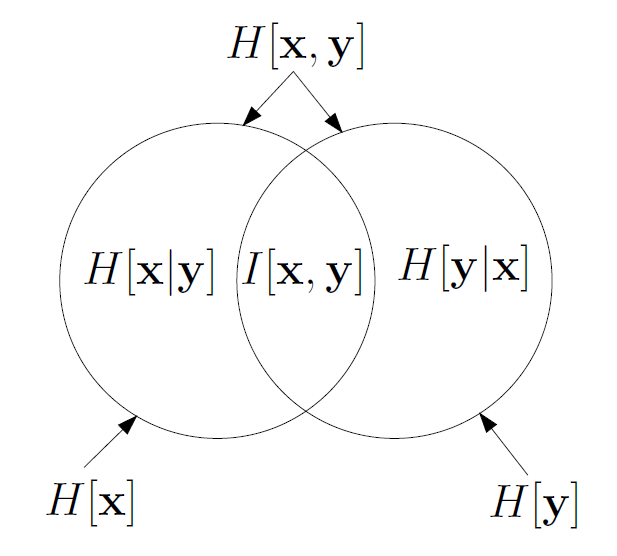
\includegraphics[width=0.7\textwidth]{./res/ch1-ex39.png} 
\caption{A diagram showing the arithmetic relationship between entropy, conditional entropy, and mutual information.} 
\label{fig:fig1} 
\end{figure}
\end{proof}

\subsection{Exercise 1.40}
\begin{proof}
\begin{align*}
\ln\left(\frac{\sum_{i=1}^Mx_i}{M}\right) &\geq \frac{1}{M}\sum_{i=1}^M\ln x_i 
= \frac{1}{M}\ln\left(\prod_{i=1}^Mx_i\right) 
= \ln\left(\prod_{i=1}^Mx_i\right)^{\frac{1}{M}},
\end{align*}
which means
\begin{align*}
\frac{\sum_{i=1}^Mx_i}{M} > \left(\prod_{i=1}^Mx_i\right)^{\frac{1}{M}},
\end{align*}
as desired.
\end{proof}

\subsection{Exercise 1.41}
\begin{proof}
\begin{align*}
I[\textbf{x},\textbf{y}] &\equiv KL(p(\textbf{x},\textbf{y})||p(\textbf{x})p(\textbf{y})) \\
&= -\iint p(\textbf{x},\textbf{y})\ln\left(\frac{p(\textbf{x})p(\textbf{y})}{p(\textbf{x},\textbf{y})}\right)d\textbf{x}d\textbf{y} \\
&= -\iint p(\textbf{x},\textbf{y})\ln\left(\frac{p(\textbf{x})}{p(\textbf{x}|\textbf{y})}\right)d\textbf{x}d\textbf{y} \\
&= -\iint p(\textbf{x},\textbf{y})\ln p(\textbf{x})d\textbf{x}d\textbf{y} + \iint p(\textbf{x},\textbf{y})\ln p(\textbf{x}|\textbf{y})d\textbf{x}d\textbf{y} \\
&= -\int p(\textbf{x})\ln \textbf{p(\textbf{x})}d\textbf{x} - H[\textbf{x}|\textbf{y}] \\
&= H[\textbf{x}] - H[\textbf{x}|\textbf{y}].
\end{align*}
By symmetry, we can get
\begin{align*}
I[\textbf{x},\textbf{y}] = H[\textbf{y}] - H[\textbf{y}|\textbf{x}],
\end{align*}
as desired.
\end{proof}
\end{document}
